\textcolor{red}{Note: this question might be confusing for students with the "none" answers for GM and PM in parts (a)-(b) depending on how unstable systems have been considered. To use, it might make sense to re-order so that it is clear that the closed-loop is unstable (from Nyquist) before asking how that impacts the GM and PM from the Bode plot. Alternatively, consider providing hints for (a) and (b) and updating the 'solnonly.'} Consider the following unity gain feedback system with Bode plot shown below. The forward gain $G(s)$ is stable. \\
%\begin{minipage}{2in}
\begin{center}
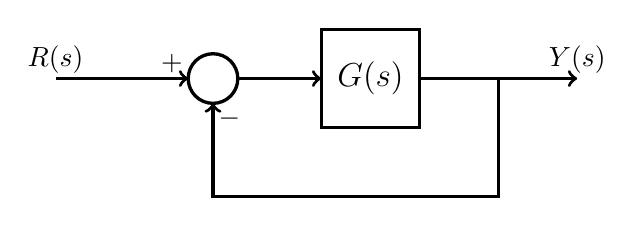
\begin{tikzpicture}[scale=1,inner sep=0pt,outer sep=0pt,very thick,
sysblock/.style={draw,rectangle,inner sep=2pt,minimum width=1.25cm,minimum height=1.25cm,inner sep=4pt, very thick}]
\draw (2,0) node[draw,circle] (sum1) {$\rule{0pt}{18pt}$};
\draw (4,0) node[sysblock] (G) {\large $G(s)$};
\draw[->] (0,0) node[above=2pt] {$R(s)$} -- (sum1.180) node[above left=2pt] {$+$};
\draw[->] (sum1.0)  -- (G.180);
\draw[->] (G.0) -- ++(2,0) node[above=2pt] {$Y(s)$};
\draw[->] (G.0) ++(1,0) -- ++(0,-1.5) -| (sum1.-90) node[below right=2pt] {$-$};
\end{tikzpicture}
\end{center}
%\end{minipage}
%\begin{minipage}{4.3in}
%The following is the Bode plot of $G(s)$, which is a stable system.
\begin{center}
\includegraphics[width=5in]{\mainfolder/LectureNotes/\lecturefolder/HomeworkProblems/Problem06/bode2.pdf}
\end{center}
%\end{minipage}
\begin{enumerate}[(a)]
\item What is the gain margin $\GMdB$?
\item What is the phase margin $\PM$?
\item Based on your knowledge of how the magnitude and phase in the Bode plot can be mapped in polar coordinates, which of the following is the correct Nyquist plot?\\
\begin{minipage}{3.25in}
\begin{enumerate}
\item[(i)]  \parbox[c]{0.5in}{\includegraphics[width=3in]{\mainfolder/LectureNotes/\lecturefolder/HomeworkProblems/Problem06/nyquist2.pdf}}
\item[(ii)]  \parbox[c]{0.5in}{\includegraphics[width=3in]{\mainfolder/LectureNotes/\lecturefolder/HomeworkProblems/Problem06/nyquist3.pdf}}
\end{enumerate}
\end{minipage}
\begin{minipage}{3in}
\begin{enumerate}
\item[(iii)]  \parbox[c]{1in}{\includegraphics[width=3in]{\mainfolder/LectureNotes/\lecturefolder/HomeworkProblems/Problem06/nyquist1.pdf}}
\item[(iv)]  \parbox[c]{1in}{\includegraphics[width=3in]{\mainfolder/LectureNotes/\lecturefolder/HomeworkProblems/Problem06/nyquist4.pdf}}
\end{enumerate}
\end{minipage}
\item Based on the Nyquist plot selected, is the closed-loop system from $R(s)$ to $Y(s)$ stable? For full credit, please show your work. 
\end{enumerate}
